\section{Results}\label{sec:findings}

\begin{figure}[h]
	\centering
	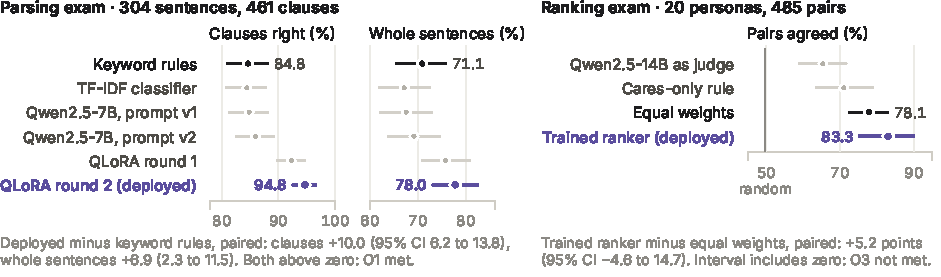
\includegraphics[width=\textwidth]{figures/fig_results.pdf}
	\caption{Both final exams (AI-written, scored once), each method with its 95\% bootstrap interval: (a,~b) parsing, (c) ranking, where the dashed line is chance. The deployed models are filled, the O1 and O3 baselines hollow black, the other methods hollow grey. Every value: Tables~\ref{tab:parse} and~\ref{tab:rank}.}
	\label{fig:results}
\end{figure}

\subsection{Parsing and Asking Back}\label{sec:res-parse}

Against the keyword-rule baseline of O1, the deployed model was \pDiffKeyC{} points better on clauses and \pDiffKeyS{} on whole sentences (paired 95\% CIs \pDiffKeyCLo{} to \pDiffKeyCHi{} and \pDiffKeySLo{} to \pDiffKeySHi; Figure~\ref{fig:results}). Fine-tuning made the difference: the same model untrained was no better than keyword rules, and training added \pDiffZeroC{} points on clauses (CI \pDiffZeroCLo{} to \pDiffZeroCHi) and \pDiffZeroS{} on whole sentences. Round~2 beat round~1 by \pDiffOneC{} points on clauses (CI \pDiffOneCLo{} to \pDiffOneCHi), but on whole sentences the difference is within noise. The offline fallback, TF-IDF with logistic regression, was chosen on validation data (\pLinVal\% of clauses against \pKeyVal\% for keywords; those clauses were mostly Chinese or mixed, the exam all English) but was no better than keyword rules on the exam; we did not switch afterwards. Splitting was exactly right for only \pSplit\% of sentences, the same for every classifier (a different split often still gives the same conditions), and most remaining sentence errors come from the rule-based steps.

The parser questioned \cAsked\% of clauses (\cAskedN, of which \cCovered{} were wrong), and \cSentWithQ\% of sentences got at least one question or offer. The questions covered \cCovered{} of the \cWrong{} wrong clauses, and for \cOption{} of them the correct reading was an option, so if students picked it clause accuracy would reach about \cProjected\% (a projection; no student answered).

\subsection{Ranking}\label{sec:res-rank}

The trained logistic regression agreed with the independent answers on \rLR\% of pairs and recovered \rLRTop{} of their top three (Table~\ref{tab:rank}); equal weights reached \rEq\% and \rEqTop. The paired difference is \rDiffEq{} points (95\% CI \rDiffEqLo{} to \rDiffEqHi), so the trained model is level with equal weights within the uncertainty: a rule that ignores what the student said does almost as well on this exam. Most of the deployed model's training pairs (\rDomShare\%) were dominance pairs, which push it towards the same choices as equal weights. The student terms helped against the teacher's labels (removing them cost \rAblInteraction{} points on 20 held-out personas) but are not shown to help on independent answers. Qwen2.5-14B judging pairs directly did worse (\rQwen\%), partly because it was asked each pair once and chose the first-shown timetable \rQwenFirst\% of the time, whereas teacher labels used both orders.

On the \rAgreePersonas{} personas answered twice, the two answerers agreed on \rAgree\% of pairs where both chose a side, similar to the human-human and human-LLM agreement of about 80\% reported in~\cite{zheng2023judge} and close to the model's score. Against the teacher's labels, accuracy was flat beyond 60 training personas, so more labels of the same kind are unlikely to help; whether better labels would is untested.

\subsection{Whole Pipeline and Reasons}\label{sec:res-pipeline}

On the parsing exam, \plExact\% of sentences (\plExactN{} of \sExamS) were parsed to exactly the intended conditions. Of the \plPlannable{} sentences whose parsed conditions allowed a timetable, \plViol{} (\plViolPct\%) received a recommendation that broke a stated condition. In half of them a clarifying question had already offered the fix, mostly hard-or-soft misreadings such as ``hates 8ams'', which the annotator treated as a limit and the parser as a preference; the rest came from splitting or number reading, such as ``no classes before 10 no classes after 4 no classes on friday'' written without commas. The first pick matched the one from the intended conditions in \plSameFirst\% of the \plSameFirstOf{} sentences where both had picks. Under the intended conditions, \plNoFit{} sentences (\plNoFitPct\%) had no timetable meeting every limit; the closest ones offered broke \plNoFitBreaks{} limits on average and never clashed (a post-freeze fallback).

All \exPicks{} template reasons passed the automatic fact check, as designed, and their main reason matched the ranker's largest contribution in \exMain\% of cases. The check's real use was on Qwen2.5-7B rewrites: only \exRewrite\% passed, and \exManualWrong{} of \exManualOf{} passed ones that Claude reviewed were still false, so the site shows templates only.

\subsection{Issues Faced}\label{sec:issue}

With the first ranking prompt, the teacher gave the same answer in both orders for only \tPilotFirst{} of \tPilotN{} pilot pairs. A side-by-side table, the main concern stated first and code-decided near-ties raised this to \tPilotAskedOK{} of the \tPilotAsked{} pairs still put to the 14B model (\tPilotFinal{} of \tPilotN{} with the code-decided ones). Students focused on waiting sometimes got more waiting, because code-labelled pairs favour fewer one-class days when waiting is equal.
